
\documentclass{standalone}

%Circular plate with distributed load
\usepackage{tikz}
\usepackage{pgfplots}
%\usepgfplotslibrary{patchplots}
%\pgfplotsset{compat=1.14}


\def\mystruct{\vphantom{hg}}

\pgfplotsset{
	legend image with text/.style={
		legend image code/.code={
		\node[anchor = center] at (0.3cm,0cm) {#1};
		}
	},width=12cm,height=7cm,compat=1.16,
}


\begin{document}



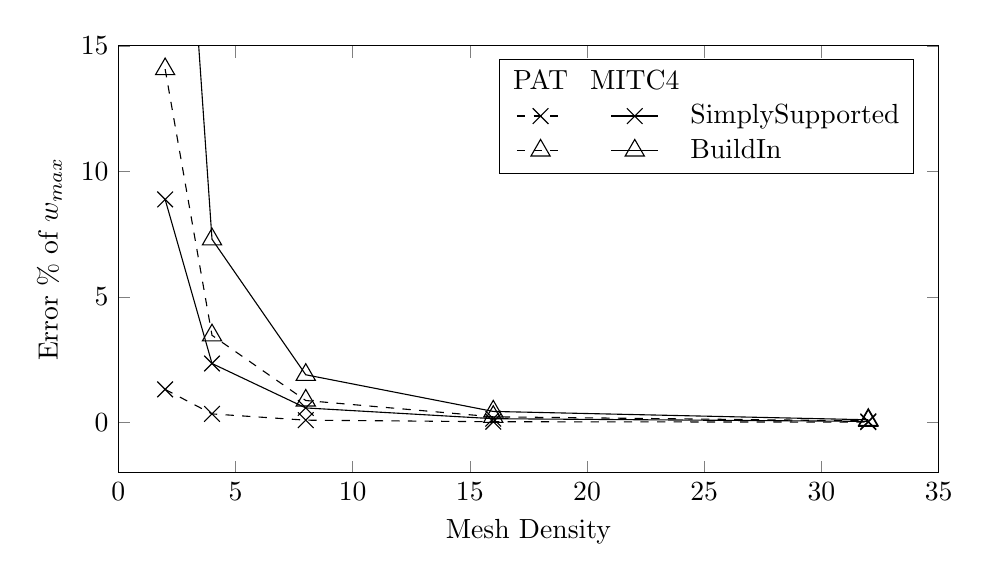
\begin{tikzpicture}
\begin{axis}[
%title={bla bla},
xlabel={Mesh Density},
ylabel={Error \% of $w_{max}$},
name=boundary,
legend columns = 2,
legend style = {
		legend cell align = left,
		},
	legend pos = north east,
	xmin=0,xmax=35,ymin=-2,ymax=15
]

\addlegendimage{legend image with text = PAT}
\addlegendentry{}

\addlegendimage{legend image with text = MITC4}
\addlegendentry{}

%C_SS_q_Tri
\addplot 
[dashed,
mark=x,mark options = {scale = 2,solid},
]
coordinates {(2,1.30963e+00)
(4,3.32870e-01)
(8,8.40844e-02)
(16,2.11104e-02)
(32,5.28751e-03)
};  \label{pgfplots:C_SS_q_Tri}
\addlegendentry{}



%C_SS_q_Rec
\addplot 
[solid,
mark=x,mark options = {scale = 2,solid},
]
coordinates {(2,8.87988e+00)
(4,2.34132e+00)
(8,5.70977e-01)
(16,1.42319e-01)
(32,3.54144e-02)

}; \label{pgfplots:C_SS_q_Rec}
\addlegendentry{SimplySupported}





%C_BI_q_Tri
\addplot 
[dashed,
mark=triangle,mark options = {scale = 2,solid},
]
coordinates {(2,1.40704e+01)
(4,3.46598e+00)
(8,8.66959e-01)
(16,2.16978e-01)
(32,5.42943e-02)


};  \label{pgfplots:C_BI_q_Tri}
\addlegendentry{}



%C_BI_q_Rec
\addplot 
[solid,
mark=triangle,mark options = {scale = 2,solid},
]
coordinates {(2,3.44336e+01)
(4,7.29104e+00)
(8,1.89246e+00)
(16,4.31397e-01)
(32,9.90850e-02)


}; \label{pgfplots:C_BI_q_Rec}
\addlegendentry{BuildIn}






%\addplot 
%[
%solid,mark options = {scale = 2,solid},
%]
%coordinates {(0,0)
%(32,0)
%};


\end{axis}

%\node [draw,fill=white,inner sep=0pt,above left = %0.5em ] at (boundary.south east) {\small
%\begin{tabular} {cc}
%fel & zdf \\
%\ref{pgfplots:C_SS_P_Tri} & %\ref{pgfplots:C_SS_P_Rec} \\
%\end{tabular}

%};


\end{tikzpicture}


\end{document}